\chapter{Jet Observables}

The next step after performing the jet clustering on the generated parton shower, is to define final state observables, that can be used to extract specific properties of the underlying physics. Here, there are two kinds of observables, event observables and jet observables.  

The most important feature of the observables is that they can be defined both for the Monte Carlo simulation and the real collision data, allowing for tuning the underlying parameters of the model used to generate the parton shower. 
\section{Single Jet Observables}

%The appropriate definition of event observables can help in forming an association between the initial stable particles and the final state particles(jets). 

%As an example of the jet observables, the following association can be made $(E, p_x, p_y, p_z)_{parton}$ $\sim$ $(E, p_x, p_y, p_z)_{jet}$. Hence, the jets were formed by combining four momentum vectors together and the jet itself is composed of multiple particles. Focusing on the first entry $E$, one can recognize that the parton energy is represented as $E_{parton}$ $\sim$ $E_{jet}$  $= \sum_{i \in jet constituents} E_{i}$,
%\Jnote{Use \textbackslash text\{\} for ``jet constituents'' in math mode.}
%where the jet constituents are the stable particles that the initially were in the event.
%\Jnote{This paragraph should be rewritten in your own words.}

An example of a jet observable is the number of the constituents in the jet with highest energy.  This gives an intuition about the formation of the jet, and allow as to tune the parameters of the parton shower.
%The histogram in figure \ref{nofcon} shows the data taken from running a jetty event 1000 times and then clustering  using anti-$k_t$ algorithm. Here, different values of the parameter $R$ were chosen.
\begin{figure}[hbtp]
\centering
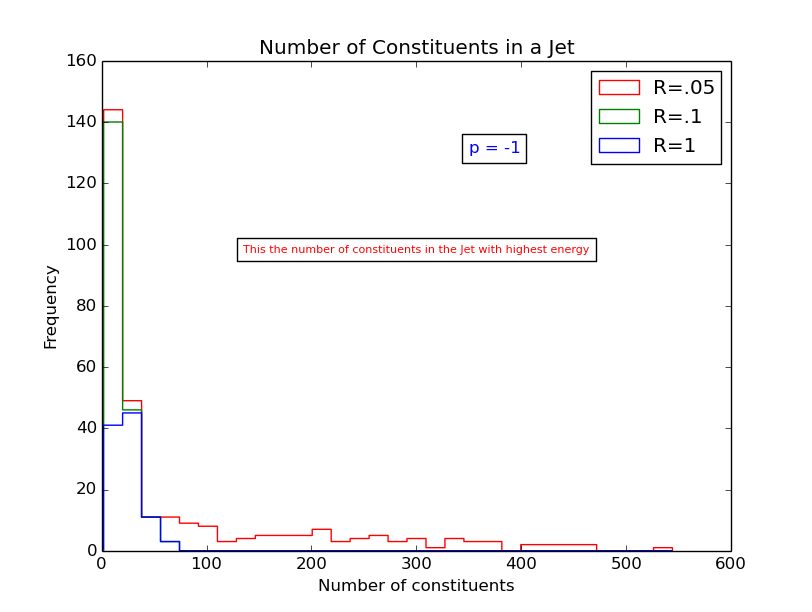
\includegraphics[scale=.8]{images/n_of_con_obs.png}
\caption{The number of constituents of a jet observable for as it is calculated different  values of $R$.  
%Note that here we are looking at the difference on the $y$ axis. The values that correspond to $R = .1$ are the differnce between the blue line $R = 1$ and maximum of $R = .1$.
}\label{nofcon}
\end{figure}

%For the code and the documentation see
%\verb+number_of_constituents_observable.py+ and for the histogram see \verb+hist_of_n_of_constituents.py+.               

Another single jet observable that we have worked on is \textit{pseudo-mass} observable. This observable is described as follows \begin{equation}
pseudo-mass(J) = E(j_1) \times E(j_2) \times \Delta_{ij} ,
\end{equation}   Where $j_1$ and $j_2$ are the two highest  momenta of of the constituents of the jet J and $\Delta_{ij}$ as given above.
%\Jnote{s/momenta/momenta of the constituents of}
%These calculations were performed on the jets with highest energy.
Conditions whenever
%\Jnote{s/Conditions where/Whenever}
the jet with the highest energy has one constituent, this observable was not calculated.


The histograms in figures \ref{nofcon} and  \ref{pseudomass} illustrate the results of this calculation for 1000 events clustered with anti-$k_t$ algorithm with different values of $R$. Where the first shows the number of constituents in a jet and the second shows the pseudo-mass observable.
%\Jnote{There are three histograms, not two.}
\begin{figure}[hbtp]
 \centering
 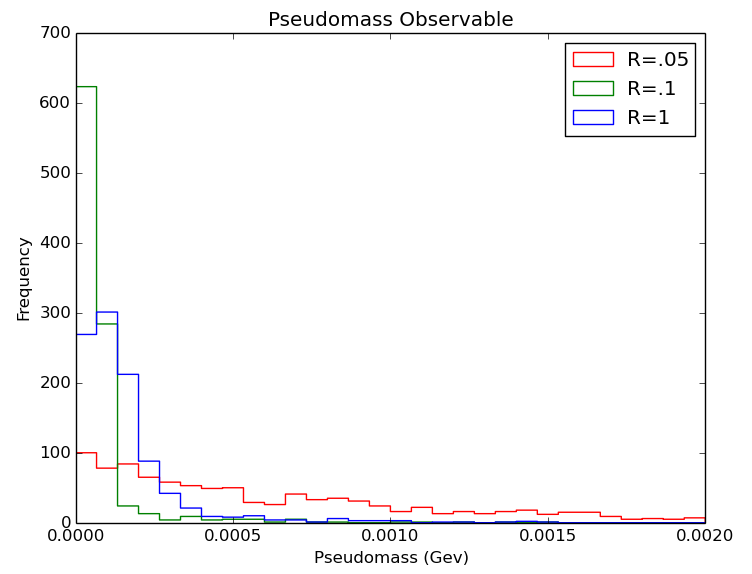
\includegraphics[scale=.65]{images/figure_13.png}
 \caption{The pseudo-mass of jet observable for different values of $R$. 
%  Note that here we are looking at the difference on the $y$ axis. The values that correspond to $R = .1$ are the differnce between the blue line $R = 1$ and maximum of $R = .1$.
}
\label{pseudomass}
\end{figure}
%
%\Jnote{Figure captions: Delete explanations about differences.}
  
%For the code and the documentation see \verb+Pseudomass_observable.py+ and for the histogram see \verb+hist_pseudomass.py+.     


\section{Event Observables} 

These observables associate the elements of initial event and final state particles (jets). An example of this is the number of jets in the event. This observable shows the number of parton that the event started with.
The histogram in figure \ref{nofjet} shows the results of clustering 1000 events using anti-$k_t$ with different values of $R$. One sees the number of jets if it is affected by the choice of $R$. It worth noting that as $R$ gets smaller, the number of jets in the event increases. 

\begin{figure}[hbtp]
 \centering
 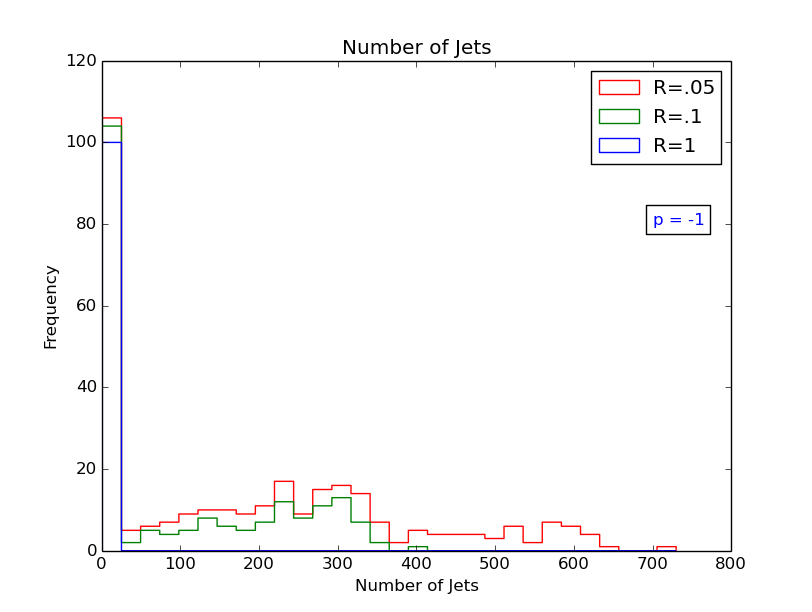
\includegraphics[scale=.8]{images/n_of_jets_obs.png}
 \caption{Number of jets for different values of $R$. Note that here we are looking at the difference on the $y$ axis. 
% The values that correspond to $R = .1$ are the differnce between the blue line $R = 1$ and maximum of $R = .1$.  
 }\label{nofjet}
 \end{figure}
  
%For the code and the documentation see \verb+number_of_Jets_observable.py+ and for the histogram see \verb+hist_n_of_Jets.py+.   
